\section{Introduction}

Nordark WP5 is digital twin-based simulation and visual analytics to assess outdoor conditions. The Nordark digital twin (DT) is a tool that support the design, planning, and assessment of suitable outdor lighting environments, as well as the specification and implementation of visual analytics tools to support data analysis. 

DT will be used for designing operations in the two study sides (pre-intervention phase) as well as supporting the analysis of results related to post-interventions. 
\begin{itemize}
    \item Pre-intervention phase: used to define the proper location and operation procedures related to both envisioned lighting solutions (WP4) as well as traps and acoustic sensors (WP3). 
    \item Post-intervention analysis: used to visualize psychological (WP1) and physiological (WP2) data collected from the different study sites. This analysis involves identifying patterns of interest, trends, and correlations with other variables, such as environment and climate data. 
\end{itemize}

The process of designing DT for intervention planning and post-intervention data analysis is illustrated in Figure \ref{Process}. The digital twin is developed using Unity with the High-Definition Rendering Pipeline (HDRP). Several Unity assets are used, the main ones being:
\begin{itemize}
    \item The Mapbox Unity SDK, to display a map of any location.
    \item Vegetation Studio Pro, to create vegetation randomly on user-defined areas.
    \item Photorealistic lights (IES), to apply IES files to lights (more on this later).
    \item A collection of vegetation assets
\end{itemize}
Detailed informartion regarding the technical documentation is provided in "Technical documentation.docsx". Additionally, the work related to the development of the digital twin is publicly available in the form of research articles, as listed in the Bibliography.


\begin{figure}[H]
    \centering
    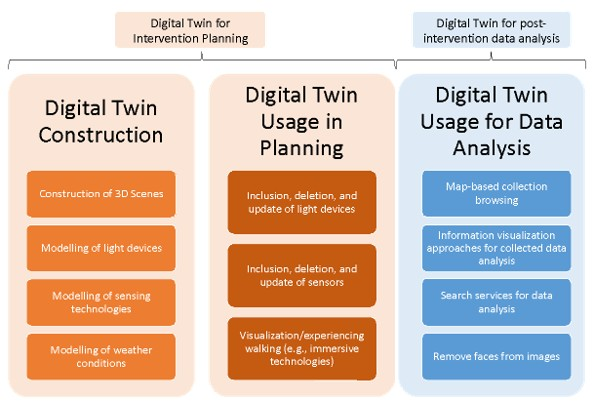
\includegraphics[width=0.8\textwidth]{Images/Process.jpg}
    \caption[The illustration of DT proces from requirement from features]{The illustration of DT proces from requirement from features}
    \label{Process}
\end{figure}

%\begin{enumerate}
    %\item Overview of the DT (the basics of how to start/run, running in full screen vs window mode etc.)
    %\item Short overview of the main functionality (brief description, details later)
    %\item Separate section/chapter pr functional area (light design, light calculations, data visualization etc)
   % \item About dataformats for files to be visualized/used by the DT
    %\begin{enumerate}
        %\item Examples of how to convert data from CSV/Excel to Geojson for the data visualisation (maybe even with some Python-scripts if we have..)
    %\end{enumerate}
    %\item Appenix: The technical document of Leo..
%\end{enumerate}




%\nocite{imt_software_wiki}  % This is an example of how to add a reference to the bibliography at the end without having it displayed as a reference within the text

\nocite{Leplat2022ECMS}
\nocite{Hassan2022ECMS}
\nocite{Leplat2022SDSC}
\nocite{Hu2023ECMS}
\nocite{Leplat2022Master}
\nocite{Hu2022Master}
\nocite{Hu2024ECMS}
\nocite{NorDark_2025}
\nocite{Afif_2024}
